\xchapter{Estudo Experimental}{}
\label{estudo-experimental}

Este capítulo apresenta o processo de avaliação utilizado para medir a precisão do
sistema de identificação de momentos oportunos e inoportunos proposto. As seções deste
capítulo estão organizadas da seguinte forma: A seção x lorem ipsum.

\section{Metodologia}
\label{metodologia}

O desempenho da proposta foi avaliado a partir de um experimento executado durante
situações reais de direção em um percurso em algumas ruas da cidade de Salvador -
Bahia. O percurso está apresentado na figura \ref{percurso}.

\begin{figure}[h]
\centering
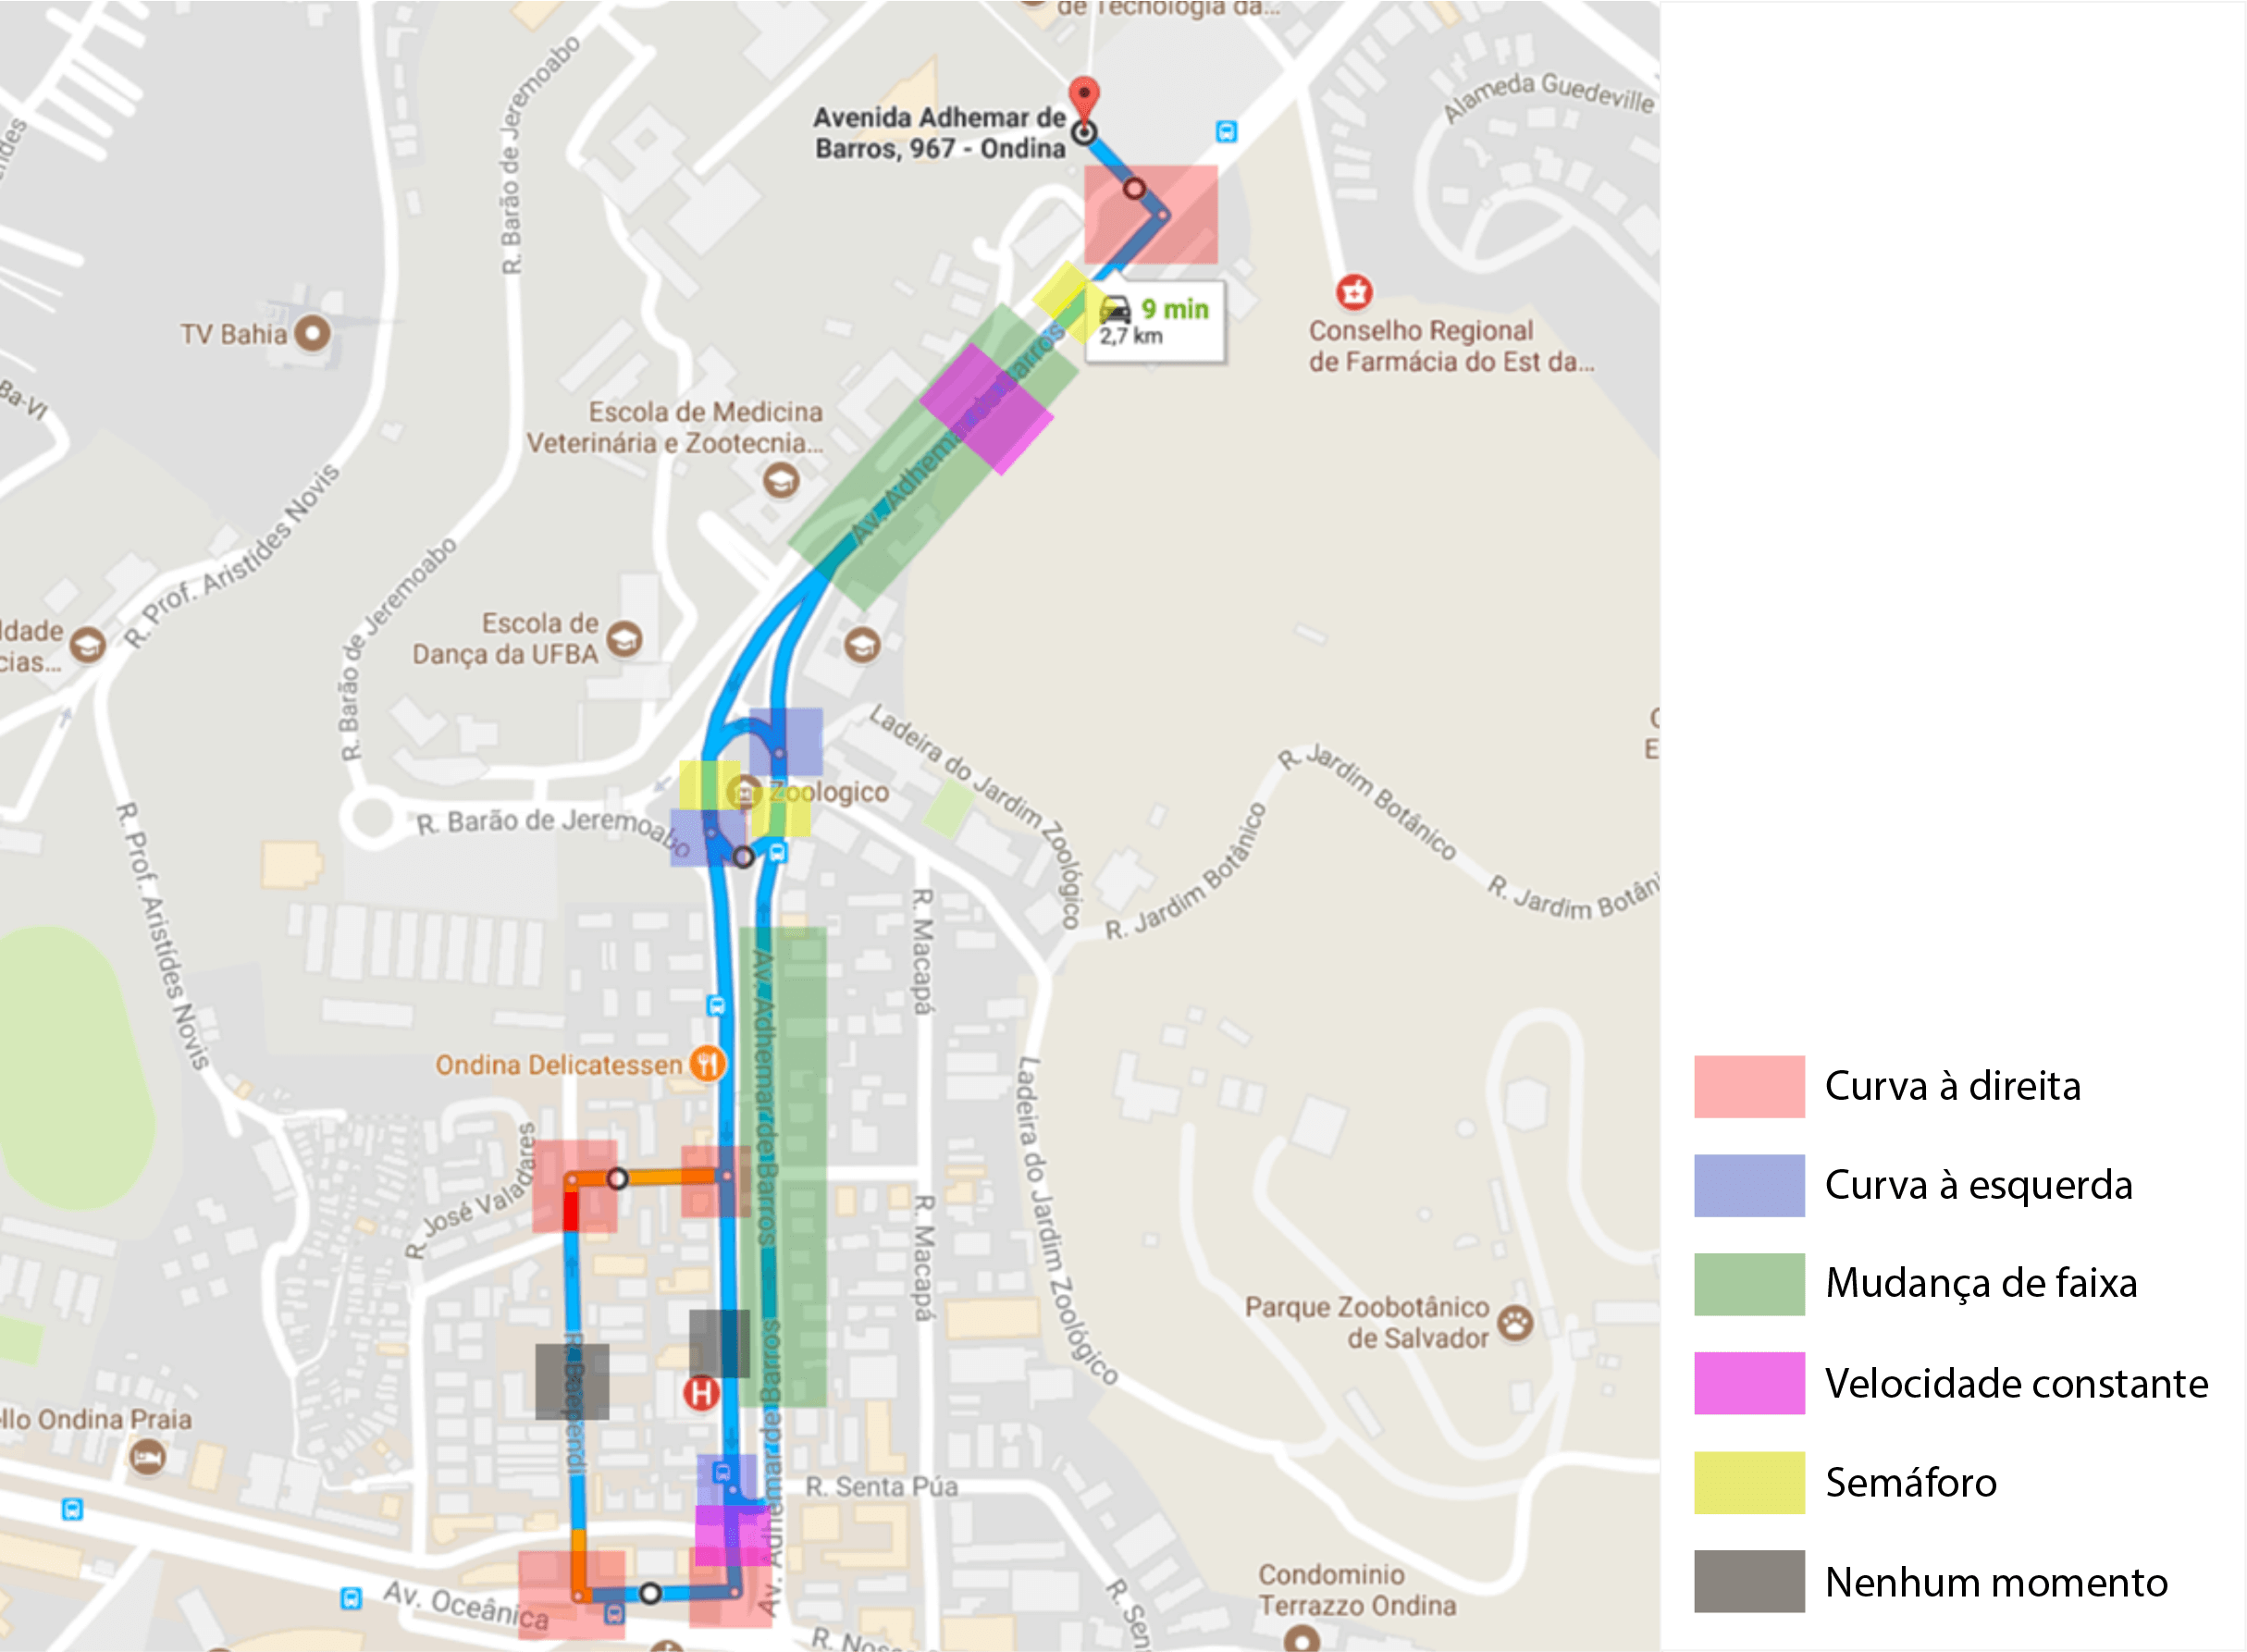
\includegraphics[width=0.53\textwidth]{images/percurso.png}
\caption{Percurso realizado no experimento de avaliação}
\label{percurso}
\end{figure}
